\documentclass[tikz,border=10pt]{standalone}
\usepackage{tikz}
\usetikzlibrary{arrows.meta,positioning}

\tikzset{
  card/.style={draw=blue!70!black, line width=1.2pt, rounded corners=3pt, minimum width=6.2cm, minimum height=1.0cm, align=center, fill=none},
  result/.style={draw=orange!80!black, line width=1.2pt, rounded corners=3pt, minimum width=6.2cm, minimum height=1.0cm, align=center, fill=none},
  flow/.style={-{Stealth[length=3mm]}, line width=1.2pt, draw=black!70}
}

\begin{document}
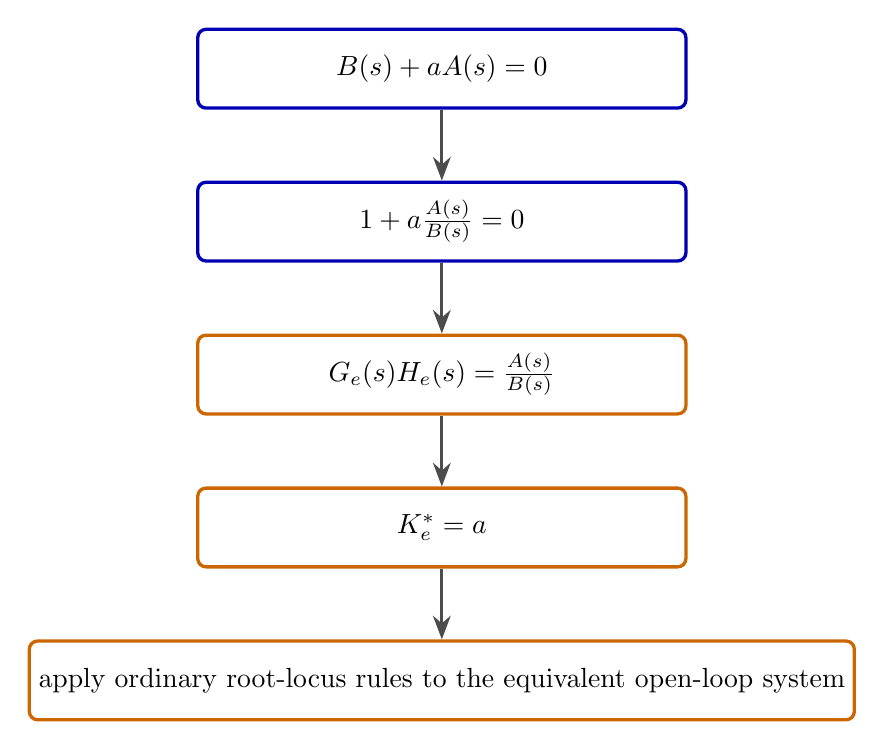
\begin{tikzpicture}[node distance=0.9cm]
  \node[card] (a) {$B(s)+aA(s)=0$};
  \node[card, below=of a] (b) {$1+a\frac{A(s)}{B(s)}=0$};
  \node[result, below=of b] (c) {$G_e(s)H_e(s)=\frac{A(s)}{B(s)}$};
  \node[result, below=of c] (d) {$K_e^\ast=a$};
  \node[result, below=of d] (e) {apply ordinary root-locus rules to the equivalent open-loop system};

  \draw[flow] (a) -- (b);
  \draw[flow] (b) -- (c);
  \draw[flow] (c) -- (d);
  \draw[flow] (d) -- (e);
\end{tikzpicture}
\end{document}
